\documentclass[border=0.8ex,svgnames,tikz]{standalone}
\usepackage{amsmath,mathtools}
\usepackage{fontspec}
\setmainfont{Source Serif 4}
\setsansfont{Source Sans 3}
\setmonofont{Source Code Pro}
\usetikzlibrary{calc,decorations.pathreplacing,matrix,patterns,tikzmark}
\usepackage{hf-tikz}
\newcommand{\matrixAColor}{Green!50!Lime!60}
\newcommand{\matrixBColor}{Orange!90}
\begin{document}
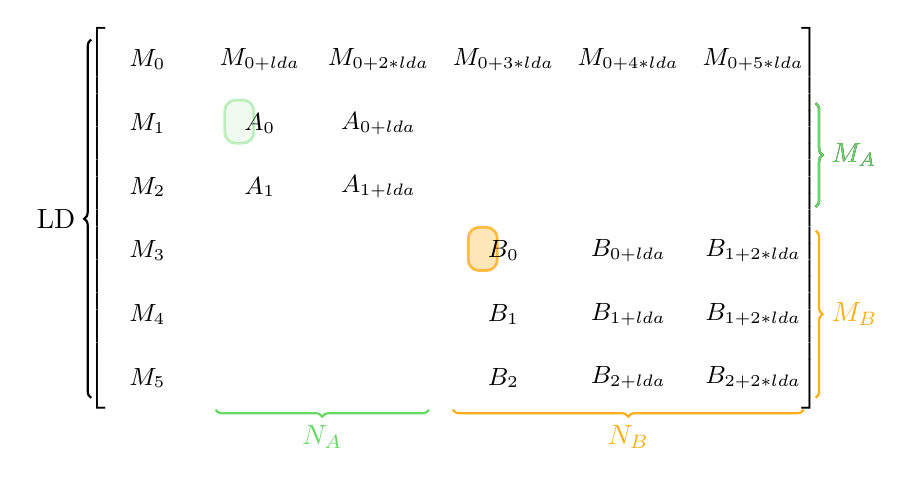
\begin{tikzpicture}[
  baseline={-1ex},
  decoration={brace},
  every left delimiter/.style={xshift=1.5ex},
  every right delimiter/.style={xshift=-1.5ex},
  ]
  \begin{scope}[
    every matrix/.style={
      matrix of math nodes,
      nodes in empty cells,
      left delimiter={[},
      right delimiter={]},
      inner sep=0.2ex,
      outer sep=0.8ex,
      column sep=2ex,
      row sep=2ex,
      nodes={
        minimum width=3.2em,
        minimum height=1.44em,
        anchor=center,
        inner sep=0pt,
        outer sep=0pt,
        font=\small,
      },
    },
    matrix A/.style={
      set fill color=\matrixAColor,draw opacity=0.4,
      set border color=\matrixAColor,fill opacity=0.1,
    },
    matrix B/.style={
      set fill color=\matrixBColor, draw opacity=0.8,
      set border color=\matrixBColor, fill opacity=0.3,
    },
    shading matrix/.style={
      above left offset={-0.25,0.25},
      below right offset={0.12,-0.30},
      #1,
    },
    set fill color/.code={\pgfkeysalso{fill=#1}},
    set border color/.style={draw=#1},
    ]
    \matrix [inner sep=0.2ex] (M) {
      M_{0} & M_{0+lda} & M_{0+2*lda} & M_{0+3*lda} & M_{0+4*lda} & M_{0+5*lda} \\
      M_{1} & \tikzmarkin[shading matrix=matrix A]{matrixA} A_{0} & A_{0+lda} & & & \\
      M_{2} & A_{1} & A_{1+lda} \tikzmarkend{matrixA} & & & \\
      M_{3} & & & \tikzmarkin[shading matrix=matrix B]{matrixB} B_{0} & B_{0+lda} & B_{1+2*lda} \\
      M_{4} & & & B_{1} & B_{1+lda} & B_{1+2*lda} \\
      M_{5} & & & B_{2} & B_{2+lda} & B_{2+2*lda} \tikzmarkend{matrixB} \\
    };
  \end{scope}
  \begin{scope}[mybrace/.style={decorate,thick,text=#1,draw=#1}]
    \draw[mybrace=Black] (M.west|-M-6-1.south west) -- node[left=2pt] {LD}
    (M.west|-M-1-1.north west);
    \draw[mybrace=Black](M.east|-M-2-1.north east) -- node[right=2pt] {$M_{A}$}
    (M.east|-M-3-1.south east);
    \draw[mybrace=\matrixAColor](M.east|-M-2-1.north east) -- node[right=2pt] {$M_{A}$}
    (M.east|-M-3-1.south east);
    \draw[mybrace=\matrixAColor](M.south-|M-1-3.north east) -- node[below=2pt] {$N_{A}$}
    (M.south-|M-1-2.north west);
    \draw[mybrace=\matrixBColor](M.east|-M-4-1.north east) -- node[right=2pt] {$M_{B}$}
    (M.east|-M-6-1.south east);
    \draw[mybrace=\matrixBColor](M.south-|M-1-6.north east) -- node[below=2pt] {$N_{B}$}
    (M.south-|M-1-4.north west);
  \end{scope}
\end{tikzpicture}
\end{document}
